% -----------------------------------------------
% Template for SMC 2009
%     smc2009.sty -> style file
% Last modified by Fabien Gouyon (smc2009@inescporto.pt)
% Modified by Juan P. Bello (ismir2008-papers@ismir.net)
% By Rainer Typke (ismir07.rainer@safersignup.com)
% Based on the 2004 template by Eloi Batlle.
% -----------------------------------------------

\documentclass{article}
\usepackage{smc2009,amsmath}
% To use when using pdflatex
\usepackage{graphicx}
\usepackage{url}
% To use when using latex, dvips and ps2pdf
% \usepackage[dvips]{graphicx}

% Title.
% ------
\title{Scores Composition based on the Guido Music Notation}

% IMPORTANT NOTICE:
% Reviews are double-blind
% Authors will not be informed of who reviews their papers, and author names will be concealed from the reviewers 
% Please avoid evident self references in the text

% Authors' names must be omitted from title page (or listed as �name(s) omitted for submission�)


% Single address
% To use with only one author or several with the same address
% ---------------
\oneauthor
 {D. Fober, C. Daudin, S. Letz, Y. Orlarey} {
 Grame - Centre national de cr\'eation musicale \\ 
\{fober, daudin, letz, orlarey\}@grame.fr
 }

\sloppy
\newenvironment{contentsmall}	{\small}
\sloppy
\newenvironment{gmnsyntax}		{\vspace{-2mm}\small}{\vspace{-2mm}}

\newcommand{\GMN}	{\emph{Guido Music Notation}}
\newcommand{\Guido}	{Guido}
\newcommand{\GAR}		{GuidoAR}
\newcommand{\syntax}[1]	{\vspace{-3mm} \small #1}
\newcommand{\code}[1]	{{\small \texttt{#1}}}
\newcommand{\gtag}[1]	{$\backslash$\code{#1}}
\newcommand{\todo}[1]	{{\\ \hspace*{-8mm} \textbf{Todo:} \texttt{#1}}}
\newcommand{\oend}		{\emph{opened-end}}
\newcommand{\obeg}		{\emph{opened-begin}}
\newcommand{\codeindent}	{\\ \hspace*{9mm}}


\begin{document}
%
\maketitle
%

\permission

\begin{abstract}
Based on the Guido Music Notation format, we have developed a library - the \GAR\ library - that provides a simple and efficient memory representation of the music notation as well as score level operations. Applying operations at score level (like cutting the score head or tail) gives raise to a set of issues related to the music notation consistency. We present the Guido Music Notation format, the \GAR\ library, the score composition operations, the music notation related issues and a proposed way to solve them.
\end{abstract}

%----------------------------------------------------------------
\section{Introduction}\label{sec:intro}
%----------------------------------------------------------------
The \Guido\ Music Notation format (GMN) \cite{hoos98} \cite{guido} has been designed by H. Hoos and K. Hamel more than ten years ago. It is very close to the Lilypond format\cite{lilypond03} \cite{lilypond06} but it has appeared before. The GMN format is a general purpose formal language for representing score level music in a platform independent plain text and human readable way. It is based on a conceptually simple but powerful formalism: its design concentrates on general musical concepts (as opposed to graphical features). A key feature of the \Guido\ design is adequacy which means that simple musical concepts are represented in a simple way and only complex notions require complex representations.

Computer music is rich of many score level music representation languages \cite{Hewlett97}\cite{Huron97}\cite{darms}\cite{SCORE}\cite{good01}. This paper doesn't aim at making a comparison between these languages and the main reason we chose the GMN format for this work is the language simplicity and readability, in combination with the availability of the Guido Engine \cite{Fober:04b}\cite{daudin09a}, a powerful open source C/C++ library for music score layout and graphic rendering based on the GMN format, providing an easy way to dynamically experiment with score level operations. 

Based on the GMN format, we have developed a C++ library, the \GAR\ library, more suitable to implement score composition operations than the Guido Engine internal memory representation. Composition operations are basic operations like transposition, cutting the head or the tail of a score, putting scores in sequence or in parallel, etc. Implementing these operations gave quickly raise to a set of issues related to the music notation consistency. To solve these issues, we propose a simple typology of the music notation elements and a set of rules based on this typology to enforce the music notation consistency.

Music notation is the most common representation used by musicians. Developing score level composition operations provides an homogeneous way to write scores and to manipulate them while remaining at a high music description level. Moreover, the design allows to use scores both as target and as arguments of the operations, enforcing the notation level metaphor.

This paper introduces first the \Guido\ Music Notation format, next the \GAR\ library is presented and the last section presents the score composition operations, the related notation issues and the proposed solution.

%----------------------------------------------------------------
\section{The Guido Music Notation format}
%----------------------------------------------------------------

\subsection{Basic concepts}
%----------------------------------------------------------------
Basic \Guido\ notation covers the representation of notes, rests, accidentals, single and multi-voiced music and the most common concepts from conventional music notation such as clefs, meter, key, slurs, ties, beaming, stem directions, etc.
Notes are specified by their name \code{(a b c d e f g h)}, optional accidentals ('\#' and '\&' for sharp and flat), an optional octave number and an optional duration. \\
Duration is specified in one of the forms: 
\begin{gmnsyntax} 
\begin{verbatim} 
   '*'enum'/'denom dotting
   '*'enum dotting 
   '/'denom dotting
\end{verbatim}
\end{gmnsyntax} 
\noindent where $enum$ and $denom$ are positive integers and $dotting$ is either empty, '.', or '..', with the same semantic than the music notation. When $enum$ or $denom$ is omitted, it is assumed to be 1. The duration represents a whole note fractional.

When omitted, optional note description parts are assumed to be equal to the previous specification before in the current sequence.

Chords are described using comma separated notes enclosed in brackets e.g \code{\{c, e, g\}}

\subsection{\Guido\ tags}
%----------------------------------------------------------------
Tags are used to represent additional musical information, such as slurs, clefs, keys, etc. A basic tag has one of the forms:
\begin{gmnsyntax} 
\begin{verbatim} 
   \tagname 
   \tagname<param-list>
\end{verbatim} 
\end{gmnsyntax}
\noindent where \code{param-list} is a list of string or numerical arguments, separated by commas (','). In addition, a tag may have a time range and be applied to a series of notes (like slurs, ties etc.); the corresponding form is:
\begin{gmnsyntax} 
\begin{verbatim} 
   \tagname(note-series)
   \tagname<param-list>(note-series)
\end{verbatim} 
\end{gmnsyntax} 

The following GMN code illustrates the concision of the notation; figure \ref{ex1} represents the corresponding \Guido\ engine output. 
\begin{gmnsyntax} 
\begin{verbatim} 
  [ \meter<"4/4"> \key<-2> c d e& f/8 g ]
\end{verbatim}
\end{gmnsyntax} 

\begin{figure}[h]
	\centering 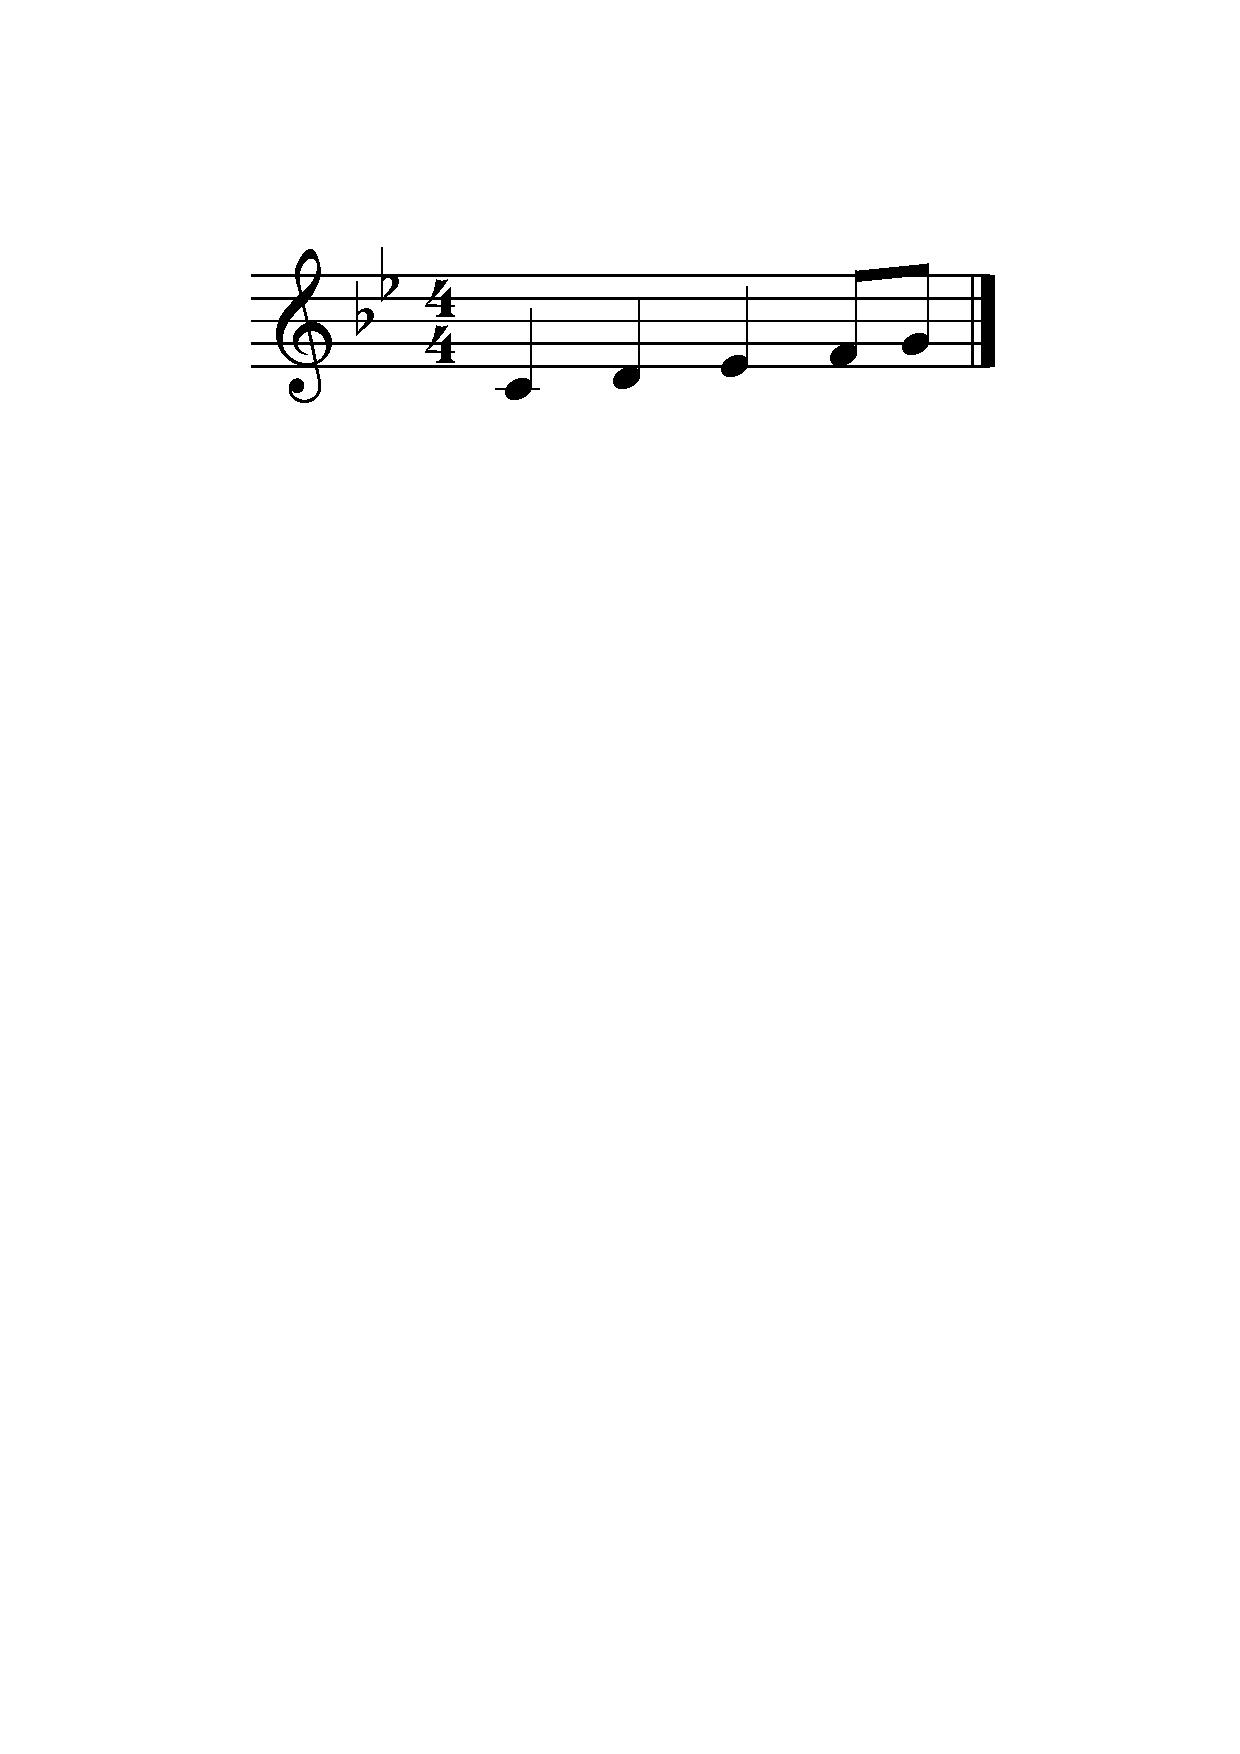
\includegraphics[width=50mm]{imgs/ex1}
 \caption{A simple GMN example}
 \label{ex1}
\end{figure}

\subsection{Notes sequences and segments}
%----------------------------------------------------------------
A note sequence is of the form \verb+[tagged-notes]+ where \code{tagged-notes} is a series of notes, tags, and tagged ranges separated by spaces. Note sequences represent single-voiced scores.
Note segments represent multi-voiced scores; they are denoted by \verb+{seq-list}+ where \code{seq-list} is a list of note sequences separated by commas as shown by the example below:
\codeindent\code{ \{ [ e g f ], [ a e a ] \} } \\
The corresponding output is given by figure \ref{ex1}.

\begin{figure}[h]
	\centering 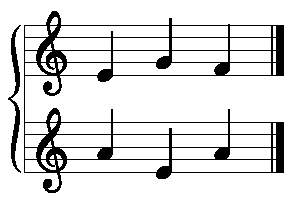
\includegraphics[width=35mm]{rsrc/voices}
 \caption{A multi-voices example}
 \label{ex1}
\end{figure}


\subsection{Advanced \Guido.}
%----------------------------------------------------------------
The advanced \Guido\ specification provides more tags and more control over the score layout.
In particular, it introduces tags parameters like $dx$ and $dy$ to indicate exact positioning of the score elements, notes and rests format specifications, staff assignments, etc. 
Below is an example of advanced guido with the corresponding output (figure \ref{advex}).

\begin{gmnsyntax} 
\begin{verbatim} 
{
 [
  \barFormat<"system">
  \staff<1> \stemsUp \meter<"2/4"> 
  \intens<"p", dx=1hs,dy=-7hs>
  \beam(g2/32 e/16 c*3/32) c/8 
  \beam(\noteFormat<dx=-0.9hs>(a1/16) c2 f) 
  \beam(g/32 d/16 h1*3/32) d2/8 
  \beam(h1/16 d2 g)],

 [\staff<1>\stemsDown g1/8 e
  \beam(f/16 \noteFormat<dx=0.8hs>(g) f a) 
   a/8 e 
  \beam(f/16 g f e)],

 [\staff<2> \meter<"2/4"> 
  \stemsUp a0 f h c1],
 [\staff<2> \stemsDown c0 d g {d, a}]
}
\end{verbatim} 
\end{gmnsyntax} 

\begin{figure}[h]
	\centering 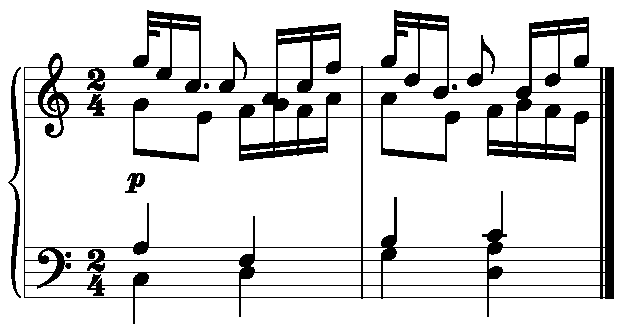
\includegraphics[width=77mm]{rsrc/4voices}
 \caption{An advanced Guido example}
 \label{advex}
\end{figure}



%----------------------------------------------------------------
\section{The GuidoAR Library}
%----------------------------------------------------------------
The \GAR\ library is a C/C++ framework providing a memory representation of the Guido Music Notation [GMN] as well as basic operations on this representation. The library name - \GAR\ - stands for Guido Abstract Representation, referring to the \Guido Engine \cite{RENZ02} \cite{Fober:04b} terminology and opposed to the Guido Graphic Representation : the abstract representation is intended as the pending memory representation of the GMN and deals with the logical score layout (stems direction, beaming, etc.) while a graphic representation is intended to provide exact graphic formatting information of the score.

The main issues in designing a C++ library to support the GMN format are related to the significant 
number of notation elements: in addition to notes, chords, voices, the format includes over hundred tags. Thus the cost of describing all the notations elements, the design of an adequate and efficient memory representation and the easiness to maintain and to manipulate have been at the center of the library design.

%----------------------------------------------------------------
\subsection{Notation elements representation}
The \GAR\ library is based on a single \code{guidoelement} class that contains a name and an attributes list (figure \ref{guidoelt}). A \code{guidoattribute} has a name, a value and an optional unit (used for exact positioning).
\begin{figure}[htbp]
	\begin{center}
	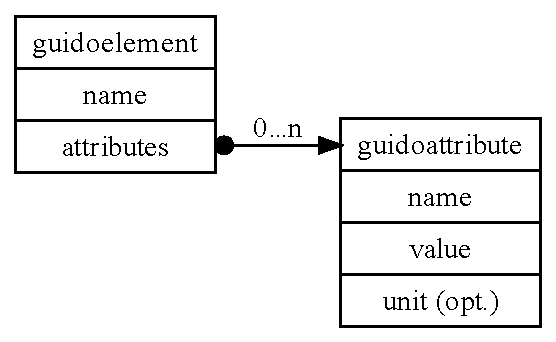
\includegraphics[width=5.2cm]{rsrc/guidoelt}
	\caption{Basic objects.}
	\label{guidoelt}
	\end{center}
\end{figure}

The  \code{guidoelement} class is specialized to represent the main elements of the notation (figure \ref{classes}). Guido tags are consistently covered by the \code{guidotag} class, derived into as many types as existing tags using templates.
\begin{figure}[htbp]
	\begin{center}
	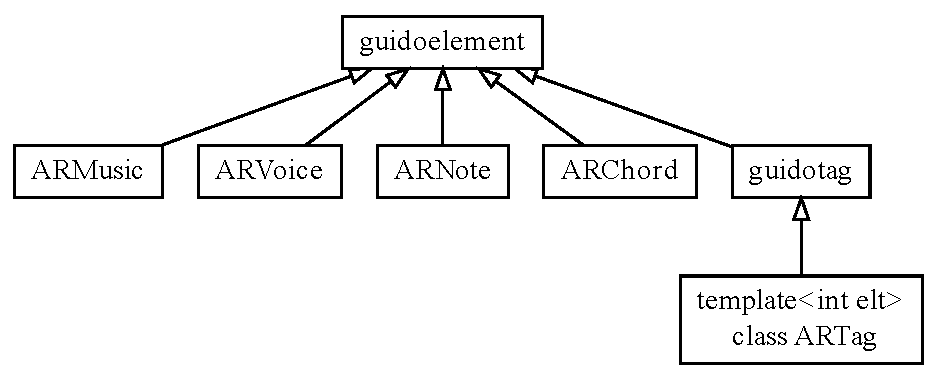
\includegraphics[width=\columnwidth]{rsrc/elements}
	\caption{The notation elements classes}
	\label{classes}
	\end{center}
\end{figure}

An automatic memory management using smart pointers simplifies the programming task. This homogeneous design leads to simplicity.

%----------------------------------------------------------------
\subsection{Browsing the representation}

The memory representation is organized into a tree similarly to the GMN hierarchy. The elements support the acyclic visitor pattern \cite{alex01} and STL iterators as well, providing simple and powerful ways to browse the music representation. The following sample code illustrates how to count the notes of a score using a visitor design: 
\begin{contentsmall} 
\begin{verbatim} 
struct countnotes : public visitor<SARNote> {
  int fCount;
        countnotes() : fCount(0)	{}
  void visitStart(SARNote&) {fCount++;}
};
\end{verbatim} 
\end{contentsmall}
And the following code implements the same feature with STL iterators and the \code{count\_if} algorithm.
\begin{contentsmall} 
\begin{verbatim} 
struct countnotespredicat {
  bool operator () (const Sguidoelement elt) 
  { return 
  	(dynamic_cast<ARNote*>((guidoelement*)elt) 
    ? true : false); }
};
countnotespredicat p;
count = count_if(score->begin(),score->end(),p);
\end{verbatim} 
\end{contentsmall}
These mechanisms are at the basis of all the score composition operations supported by the library.

%----------------------------------------------------------------
\section{Scores Composition}
%----------------------------------------------------------------

%----------------------------------------------------------------
\subsection{Basic operations}
Score level operations provided by the \GAR\ library are given by the table \ref{operations}. These operations are available as library API calls and as command line tools as well. Almost all of the operations take a GMN score and a value parameter as input and produce a GMN score as output, but the value parameter can also be indicated using another GMN score.
For example, the \code{guidotop} operation cuts the bottom voices of a score after a given voice number; when using a score as parameter, the voice number is taken from the score voices count.

\begin{table*}[htdp]
\caption{Score level operations}
\begin{center}
\begin{tabular}{rl}
tool name and args		&	description \\
\hline
guidoseq $s1\ s2$		& puts the scores $s1$ and $s2$ in sequence \\
guidopar $s1\ s2$		& puts the scores $s1$ and $s2$ in parallel \\ 
guidorpar $s1\ s2$		& puts the scores $s1$ and $s2$ in parallel but right aligned \\
guidotop $s1\ [n\ | \ s2]$ 	& takes the $n$ top voices of $s1$; \\
					& when using a score $s2$ as parameter, $n$ is taken from $s2$ voices count \\
guidobottom $s1\ [n\ | \ s2]$ 	& takes the bottom voices of $s1$ after the $n$ voice;  \\
					& when using a score $s2$ as parameter, $n$ is taken from $s2$ voices count \\
guidohead	$s1\ [d\ | \ s2]$	& takes the head of $s1$ up to the date $d$; \\
				& when using a score $s2$ as parameter, $d$ is taken from $s2$ duration \\
guidoevhead $s1\ [n\ | \ s2]$	& id. but on events basis i.e. the cut point is specified in $n$ events count; \\
				& when using a score $s2$ as parameter, $n$ is taken from $s2$ events count \\
guidotail	$s1\ [d\ | \ s2]$ 	& takes the tail of a score after the date $d$; \\
				& when using a score $s2$ as parameter, $d$ is taken from $s2$ duration \\
guidoevtail $s1\ [n\ | \ s2]$ 	& id. but on events basis i.e. the cut point is specified in $n$ events count; \\
				& when using a score $s2$ as parameter, $n$ is taken from $s2$ events count \\
guidotranspose $s1\ [i\ | \ s2]$	& transposes $s1$ to an interval $i$; \\
				& when using a score $s2$ as parameter, $i$ is computed as the difference between \\
				& the first voice, first notes of $s1$ and $s2$ \\
guidoduration $s1\ [d\ |\ f\ |\ s2]$	& stretches $s1$ to a duration $d$ or using a factor $f$; \\
				& when using a score $s2$ as parameter, $d$ is computed from $s2$ duration \\
guidoapplypitch $s1\ s2$	& applies the pitches of $s1$ to $s2$; \\
				& the pitches list is applied in a loop up to the end of $s2$ \\
guidoapplyrythm $s1\ s2$	& applies the rhythm of $s1$ to $s2$; \\
				& the durations list is applied in a loop up to the end of $s2$ \\
\hline
\end{tabular}
\end{center}
\label{operations}
\end{table*}

%----------------------------------------------------------------
\subsection{Notation issues}
Actually and to preserve the notation consistency, most of the score level operations are more complex than simply cutting or adding a branch in the memory representation. We'll illustrate the problem with the textual representation which is equivalent to the memory representation.
Let's take the example of the \code{tail} operation with the following simple score: 
\codeindent \code{[\gtag{clef}<"f"> c d e c]}\\
A raw cut of the score after 2 notes would give the \code{[\ e\ c]} result which would be naturally rendered as illustrated by the figure \ref{ex2} while the use of the same clef is expected.
\begin{figure}[h]
	\centering 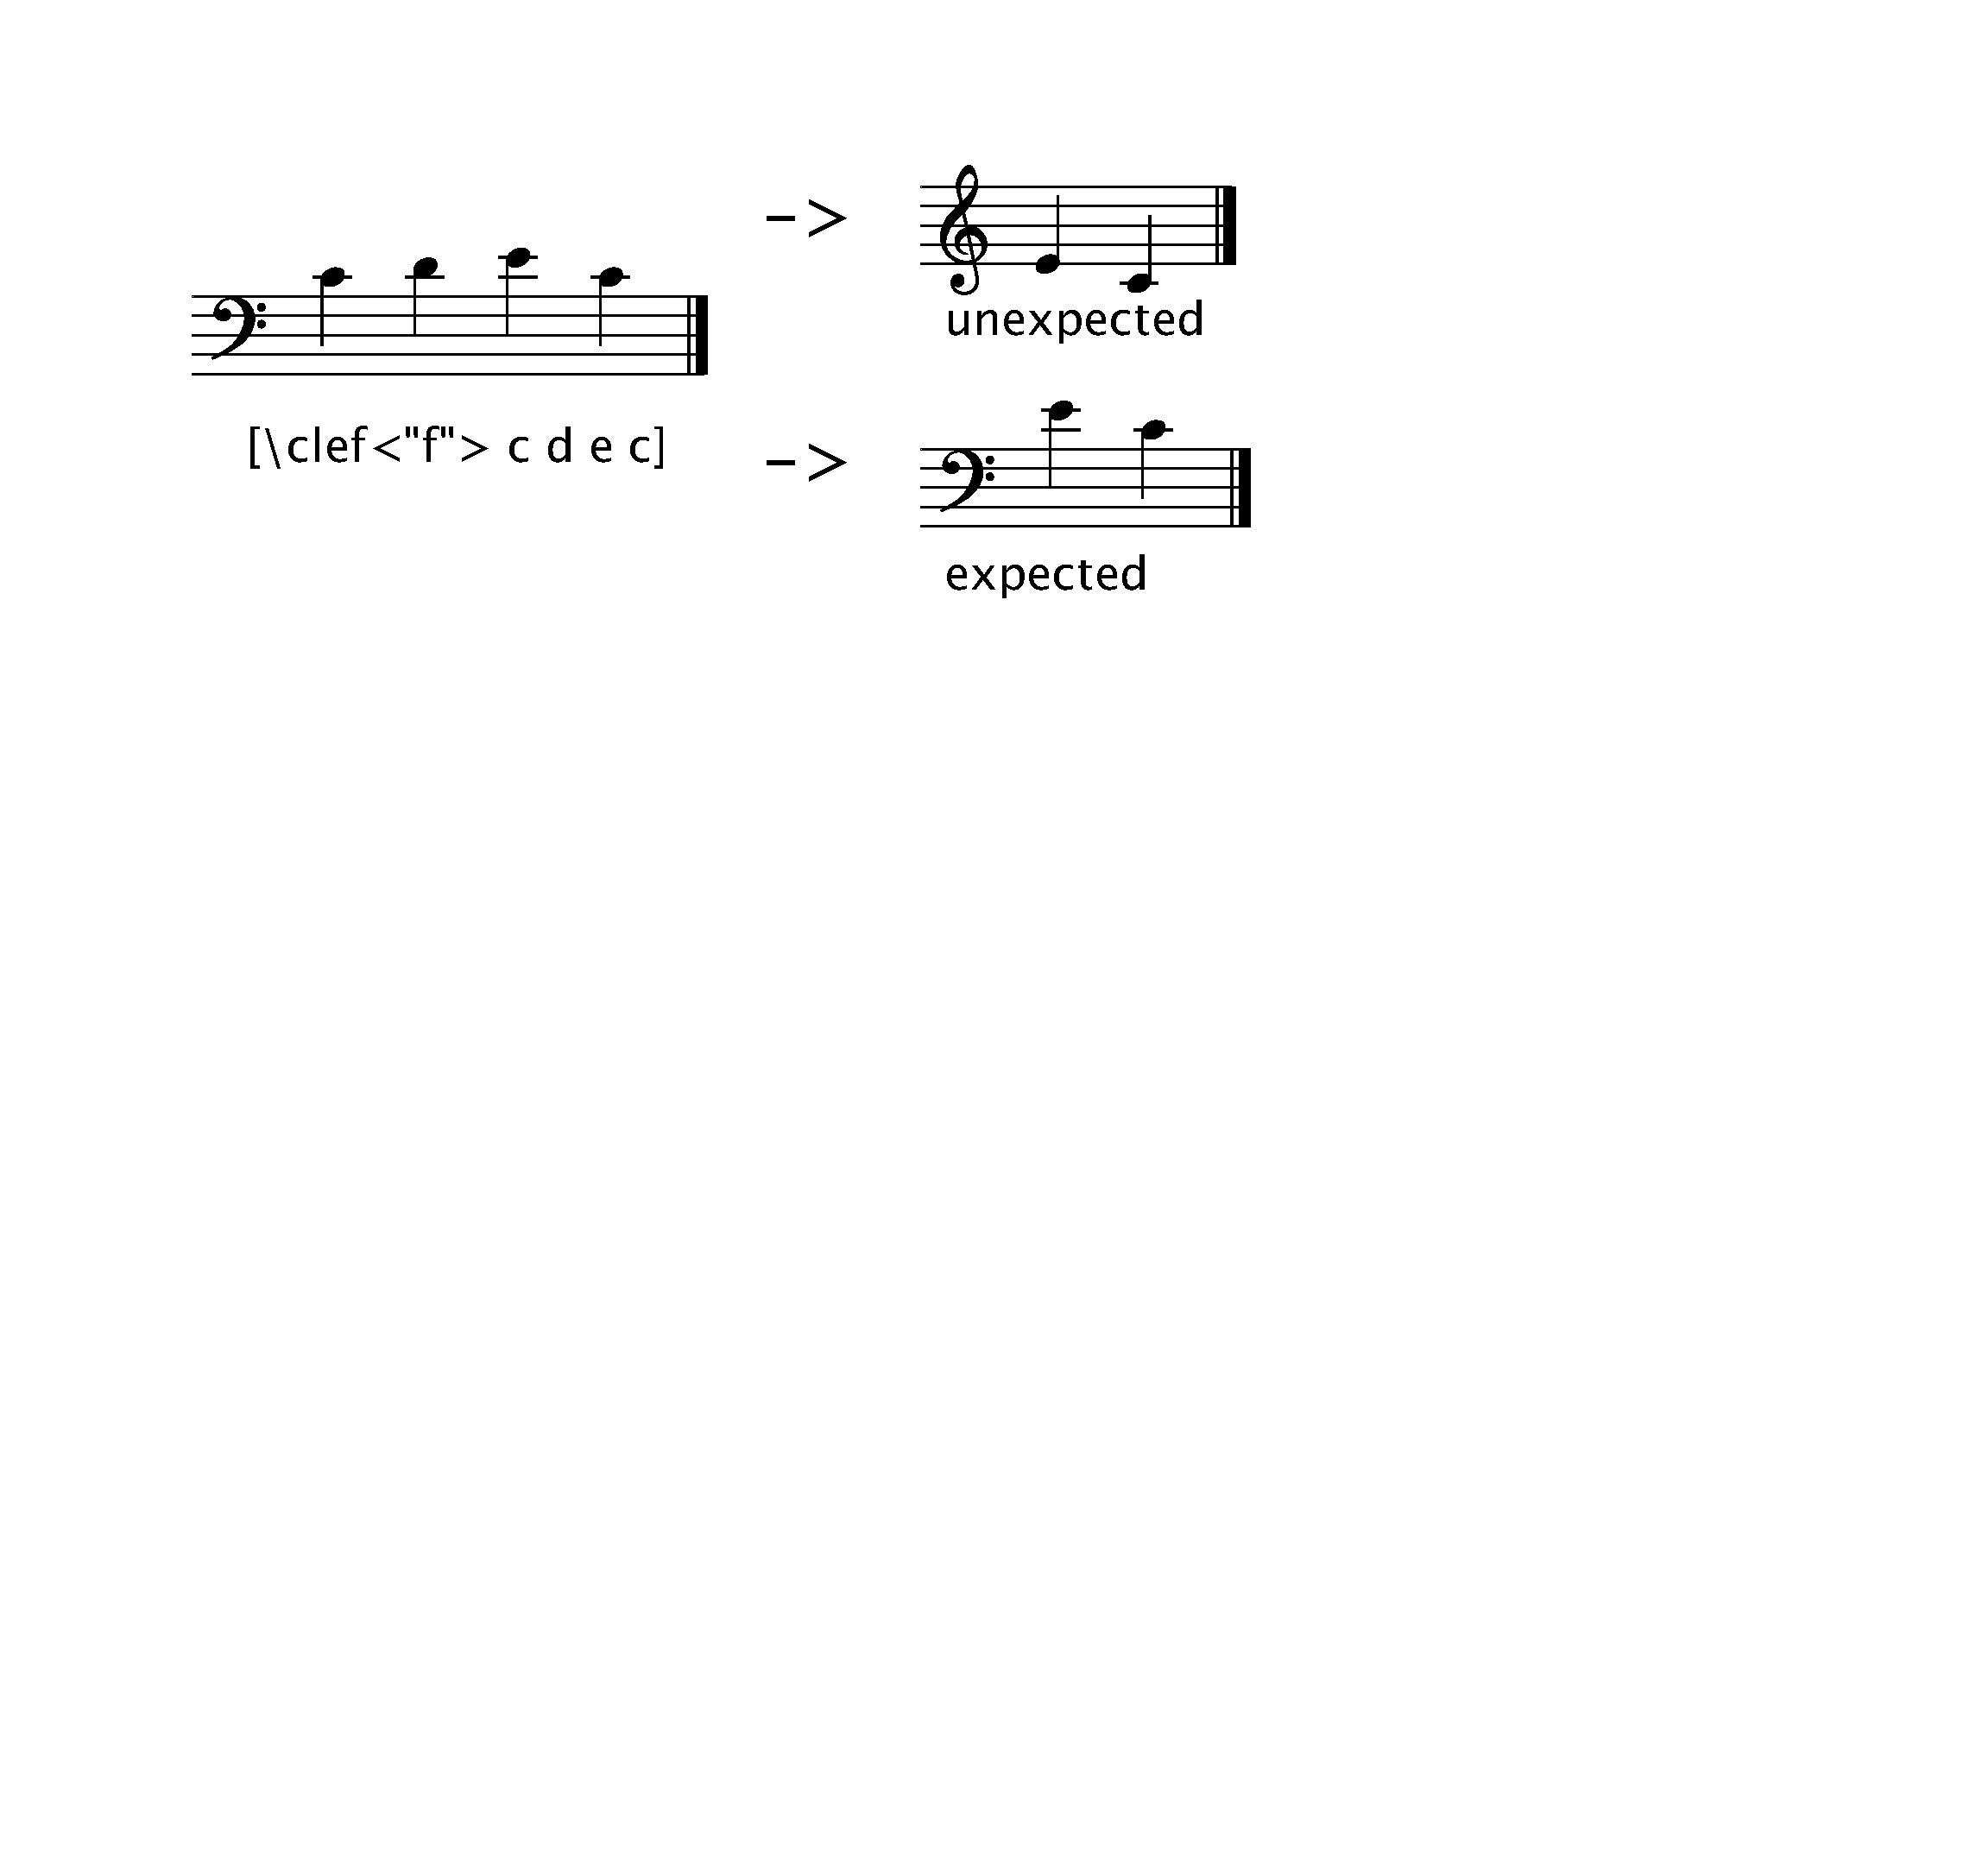
\includegraphics[width=60mm]{imgs/tail}
 \caption{Tail operation consistency}
 \label{ex2}
\end{figure}

Another example with the \code{sequence} operation: a raw sequence of 
\hspace{2mm} \code{[\gtag{clef}<"g"> c d]} \\
and \hspace{14.5mm}\code{[\gtag{clef}<"g"> e c]} \\
would give \hspace{3.1mm} \code{[\gtag{clef}<"g"> c d \gtag{clef}<"g"> e c ]} as result (figure \ref{ex3}) while the clef repetition is unexpected.
\begin{figure}[h]
	\centering 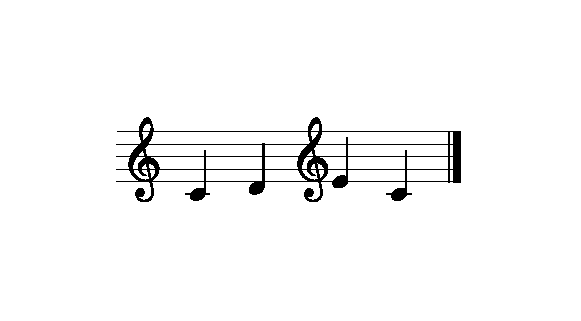
\includegraphics[width=40mm]{imgs/seq2}
 \caption{A raw sequence operation}
 \label{ex3}
\end{figure}

Some operations may also result in syntactically incorrect results. Consider the following code:
\codeindent \code{[g \gtag{slur}(f e) c]} \\
slicing the score in 2 parts after \code{f} would result in 
\codeindent \code{[g \gtag{slur}(f]} (a) \ \  and \ \  \code{[e) c]} (b) \\
i.e. with uncompleted range tags. We'll further use the terms \oend\ tags to refer the a) form and \obeg\ tags for the b) form.

There are many more cases, where the music notation consistency has to be preserved through scores composition operations.

%----------------------------------------------------------------
\subsection{Notation elements time extend}
One way to solve the problem is to make a typology of the notation elements regarding their time extend and to define adequate consistency policies according to the operations and the element type.

The GMN format makes a distinction between \emph{position} tags (like \gtag{clef} or \gtag{meter}) and \emph{range} tags (\gtag{slur}, \gtag{beam}, etc.): range tags have an explicit time extend (the duration of the enclosed notes) and position tags are simply notations marks at a given time position. However, this distinction is not sufficient to cover the problem: many of the position tags have an implicit time duration and they generally last up to the next similar notation or to the end of the score. For example, a \gtag{meter} tag lasts to the end of the score or to the next meter notation.
\begin{table}[htdp]
\caption{Typology of notation elements.}
\begin{center}
\begin{tabular}{cll}
time extend & description & sample \\
\hline
explicit 	& duration is explicit 	& slurs, cresc. \\
			& from the notation		& etc. \\
implicit 	& element lasts to the	& meter, clef, \\
			& end of the score or to	& key, etc. \\
			& the next similar element	& \\
others 		& structure control	& coda, da capo, \\
			& 	& repeats, etc. \\
	 		& formatting instructions	& new line, \\
			& 	& new page, etc. \\
	 		& notation marks	& breath mark, \\
			& 	& bar, etc. \\
\hline
\end{tabular}
\end{center}
\label{types}
\end{table}
The table \ref{types} presents a simple typology of the music notation elements.
All the Guido range tags correspond to the explicit time extend elements and most of the position tags have an implicit time extend. Based on this typology, a set of simple rules for score level operations could partially solve the notation issues:
\begin{itemize}
\item when computing the end of a score, all the explicit time extend elements must be properly closed,
\item when computing the beginning of a score, all the pending explicit time extend elements (i.e. \obeg\ tags) must be recalled,
\item when computing the beginning of a score, all the current implicit time extend elements must be recalled,
\item when putting scores in sequence, implicit time extend elements starting the second score must be skipped when they correspond to current existing elements.
\end{itemize}
No provision is made for the notation elements falling into the \emph{other} time extend category except for the \emph{structure control} elements (see section \ref{sc}).

%----------------------------------------------------------------
\subsection{Operations reversibility}\label{reverse}
The above rules solve most of the notation consistency issues but they do not permit the operations to be reversible. Consider a score including a slur, sliced in the middle of this slur and restored by putting the parts back in sequence. The resulting score will include two slurs (figure \ref{ex4}) instead one, due to the rules that enforce closing \oend\ tags and starting \obeg\ tags.

\begin{figure}[h]
	\centering 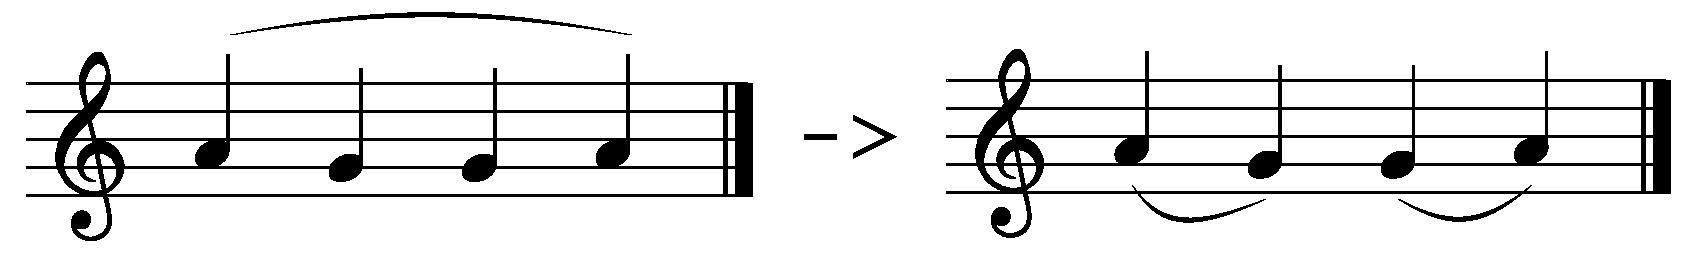
\includegraphics[width=80mm]{imgs/reverse}
 \caption{A score sliced and put back in sequence}
 \label{ex4}
\end{figure}

Here to solve the problem, we'll need the support of the GMN language. The idea is to keep the history of the range tags by introducing a new tag parameter to indicate tags creation corresponding to \oend\ and \obeg\ tags. The parameter has the form: 
\codeindent \code{\gtag{tag}<open="type">} 
\codeindent where \code{open} is the parameter name
\codeindent and \code{type} is between \code{begin} and \code{end} \\
corresponding respectively to \obeg\ and \oend\ tags.
Next, we introduce a new rule for score level operations. Let's first define \emph{adjacent} tags as tags placed on the same voice and not separated by any note or chord.
\begin{itemize}
\item \emph{adjacent} similar tags carrying an \code{open} parameter are mutually cancelled when the first one is \oend\ and the second one \obeg .
\end{itemize}
Thus when a score level operation encounters a form like: \\
\hspace*{-2mm}\code{\gtag{tag}<open="end">(f g) \gtag{tag}<open="begin">(f e)} \\
it should transform it to:
\codeindent \code{\gtag{tag}(f g f e)} \\
which solves the reversibility issue.

%----------------------------------------------------------------
\subsection{Structure control issues} \label{sc}
Elements relevant to the \emph{others / structure control} time extend category may also give rise to inconsistent notation: a \emph{repeat begin} bar without \emph{repeat end}, a \emph{dal segno} without \emph{segno}, a \emph{da capo al fine} without \emph{fine}, etc. We introduce 2 new rules to catch the repeat bars issue. Let's first define a \emph{pending} repeat end as the case of a voice with a repeat begin tag without matching repeat end.
\begin{itemize}
\item when computing the end of a score, every \emph{pending} repeat end must be closed with a repeat end tag.
\item from successive unmatched repeat begin tags, only the first one must be retained and from successive repeat end tags, only the last one must be retained.
\end{itemize}
No additional provision is made for the other structure control elements: possible inconsistencies are ignored but this choice preserves the operations reversibility.

%----------------------------------------------------------------
\section{Conclusion}
%----------------------------------------------------------------
Music notation is complex due to the large number of notation elements and to the heterogeneous status of these elements. The proposed typology in table \ref{types} is actually an arbitrary simplification intended to cover the needs of score level operations but is not representative of this complexity. However, it is based on the music notation semantic and thus could be reused with any score level music representation language. Apart from the reversibility rules defined in \ref{reverse} that require the support of the music representation language to operate, all the other rules are independent from the GMN format.
Most of the elements relevant to the \emph{others} time extend category have been ignored by the proposed rules, which may result in \emph{non-standard} layout (e.g. incoherent formatting instructions), but it preserves the operations reversibility. Thus the score composition operations do not guaranty a correct automatic music layout. 
%but they proved to be very convenient for basic tasks like taking an excerpt of a score, separating voices, etc.
In a future work, we plan to transform the notation into a lambda calculus based programming language \cite{Orlarey:94} with these operations as language operators.
%which is often a matter of user choice and also remains the Holy Grail quest of music notation by computer up to now\cite{BIRD84}.

\bibliographystyle{unsrt}
\bibliography{smc2009}

\end{document}
